\documentclass[12pt,twoside]{report}

% some definitions for the title page
\newcommand{\reporttitle}{Transfer Learning for Deep Learning Radiotherapy Planning}
\newcommand{\reportauthor}{Anton Zhitomirsky}
\newcommand{\supervisor}{Prof Ben Glocker}
\newcommand{\secondMarker}{Dr Thomas Heinis}
\newcommand{\reporttype}{MEng Individual Project}

% load some definitions and default packages
%%%%%%%%%%%%%%%%%%%%%%%%%%%%%%%%%%%%%%%%%
% University Assignment Title Page 
% LaTeX Template
% Version 1.0 (27/12/12)
%
% This template has been downloaded from:
% http://www.LaTeXTemplates.com
%
% Original author:
% WikiBooks (http://en.wikibooks.org/wiki/LaTeX/Title_Creation)
%
% License:
% CC BY-NC-SA 3.0 (http://creativecommons.org/licenses/by-nc-sa/3.0/)
% 
%
%%%%%%%%%%%%%%%%%%%%%%%%%%%%%%%%%%%%%%%%%
%----------------------------------------------------------------------------------------
%	PACKAGES AND OTHER DOCUMENT CONFIGURATIONS
%----------------------------------------------------------------------------------------
\usepackage[a4paper,hmargin=2.0cm,vmargin=1.0cm,includeheadfoot]{geometry}
\usepackage{textpos}

\usepackage[square,numbers]{natbib} % for bibliography
\usepackage[nottoc]{tocbibind} % Includes "References" in the table of contents
\bibliographystyle{unsrtnat}

\usepackage{tabularx,longtable,multirow,subfigure,caption}%hangcaption
\usepackage{fancyhdr} % page layout
\usepackage{url} % URLs
\usepackage[english]{babel}
\usepackage{amsmath}
\usepackage{graphicx}
\usepackage{scalerel}
\usepackage{dsfont}
\usepackage{epstopdf} % automatically replace .eps with .pdf in graphics
\usepackage{backref} % needed for citations
\usepackage{array}
\usepackage{latexsym}

\usepackage[pdftex,pagebackref,hypertexnames=false,colorlinks]{hyperref} % provide links in pdf
\usepackage{booktabs}
\usepackage{wrapfig}
\usepackage{caption}  % Required for \captionof
\usepackage{float} % for H option in figures
\usepackage{amssymb}
\usepackage{amsmath}
\usepackage{csquotes}
% \usepackage{subcaption} % causes a compilation error after changing back to natbib referencing... 

\hypersetup{pdftitle={},
  pdfsubject={}, 
  pdfauthor={},
  pdfkeywords={}, 
  pdfstartview=FitH,
  pdfpagemode={UseOutlines},% None, FullScreen, UseOutlines
  bookmarksnumbered=true, bookmarksopen=true, colorlinks,
    citecolor=black,%
    filecolor=black,%
    linkcolor=black,%
    urlcolor=black}

\usepackage[all]{hypcap}

%%%%%%%%%%%%%%%%%%%%%%%%%%%%%%%%%%%%%%%%%%%%%%%%%%%%%%%%%%%%%%%%%%%%%%%%%%%%%%%%
% LISTINGS ammendments
%%%%%%%%%%%%%%%%%%%%%%%%%%%%%%%%%%%%%%%%%%%%%%%%%%%%%%%%%%%%%%%%%%%%%%%%%%%%%%%%
\usepackage{listings}

\lstset
{ %Formatting for code in appendix
    language=Matlab,
    basicstyle=\footnotesize,
    % numbers=left,
    stepnumber=1,
    showstringspaces=false,
    tabsize=1,
    breaklines=true,
    breakatwhitespace=false,
    frame=single,
    columns=fullflexible,
    postbreak=\mbox{\textcolor{red}{$\hookrightarrow$}\space},
}

%\usepackage{color}
%\usepackage[tight,ugly]{units}
%\usepackage{float}
%\usepackage{tcolorbox}
%\usepackage[colorinlistoftodos]{todonotes}
% \usepackage{ntheorem}
% \theoremstyle{break}
% \newtheorem{lemma}{Lemma}
% \newtheorem{theorem}{Theorem}
% \newtheorem{remark}{Remark}
% \newtheorem{definition}{Definition}
% \newtheorem{proof}{Proof}


%%% Default fonts
\renewcommand*{\rmdefault}{bch}
\renewcommand*{\ttdefault}{cmtt}


%%% Default settings (page layout)
\setlength{\parindent}{0em}  % indentation of paragraph
\setlength{\parskip}{.3em}

% \setlength{\parindent}{0em}  % indentation of paragraph

\setlength{\headheight}{14.5pt}
\pagestyle{fancy}
\renewcommand{\chaptermark}[1]{\markboth{\chaptername\ \thechapter.\ #1}{}}
%\fancyhead[RO]{\sffamily \textbf{\thepage}} %Page no.in the right on even pages
%\fancyhead[LE]{\sffamily \textbf{\thepage}} %Page no. in the left on odd pages

\fancyfoot[ER,OL]{\thepage}%Page no. in the left on
%odd pages and on right on even pages
\fancyfoot[OC,EC]{\sffamily }
\renewcommand{\headrulewidth}{0.1pt}
\renewcommand{\footrulewidth}{0.1pt}
\captionsetup{margin=10pt,font=small,labelfont=bf}


%--- chapter heading

\def\@makechapterhead#1{%
  \vspace*{10\p@}%
  {\parindent \z@ \raggedright \sffamily
    \interlinepenalty\@M
    \Huge\bfseries \thechapter \space\space #1\par\nobreak
    \vskip 30\p@
  }}

%--- chapter heading

\def\@makechapterhead#1{%
  \vspace*{10\p@}%
  {\parindent \z@ \raggedright \sffamily
    %{\Large \MakeUppercase{\@chapapp} \space \thechapter}
    %\\
    %\hrulefill
    %\par\nobreak
    %\vskip 10\p@
    \interlinepenalty\@M
    \Huge\bfseries \thechapter \space\space #1\par\nobreak
    \vskip 30\p@
  }}

%---chapter heading for \chapter*  
\def\@makeschapterhead#1{%
  \vspace*{10\p@}%
  {\parindent \z@ \raggedright
    \sffamily
    \interlinepenalty\@M
    \Huge \bfseries  #1\par\nobreak
    \vskip 30\p@
  }}
\allowdisplaybreaks

% load some macros
% Here, you can define your own macros. Some examples are given below.

\newcommand{\R}[0]{\mathds{R}} % real numbers
\newcommand{\Z}[0]{\mathds{Z}} % integers
\newcommand{\N}[0]{\mathds{N}} % natural numbers
\newcommand{\C}[0]{\mathds{C}} % complex numbers
% \renewcommand{\vec}[1]{{\boldsymbol{{#1}}}} % vector
\newcommand{\mat}[1]{{\boldsymbol{{#1}}}} % matrix

\usepackage{pifont,mdframed}
\newenvironment{warning}
  {\par\begin{mdframed}[linewidth=1pt,linecolor=black]%
    \begin{list}{}{\leftmargin=1cm
                  \labelwidth=\leftmargin}\item[\Large\ding{43}]}
  {\end{list}\end{mdframed}\par}

\definecolor{lightgray}{gray}{0.9}

% load title page
\begin{document}
% Last modification: 2015-08-17 (Marc Deisenroth)
\begin{titlepage}

    \newcommand{\HRule}{\rule{\linewidth}{0.5mm}} % Defines a new command for the horizontal lines, change thickness here
    
    %----------------------------------------------------------------------------------------
    %	LOGO SECTION
    %----------------------------------------------------------------------------------------
    
    
\includegraphics[width = 4cm]{../figures/imperial.pdf}\\[0.5cm] 
    
    \center % Center everything on the page
     
    %----------------------------------------------------------------------------------------
    %	HEADING SECTIONS
    %----------------------------------------------------------------------------------------
    
    \textsc{\LARGE \reporttype}\\[1.5cm] 
    \textsc{\Large Department of Computing}\\[0.5cm] 
    \textsc{\large Imperial College of Science, Technology and Medicine}\\[0.5cm] 
    
    %----------------------------------------------------------------------------------------
    %	TITLE SECTION
    %----------------------------------------------------------------------------------------
    
    \HRule \\[0.4cm]
    { \huge \bfseries \reporttitle}\\ % Title of your document
    \HRule \\[1.5cm]
     
    %----------------------------------------------------------------------------------------
    %	AUTHOR SECTION
    %----------------------------------------------------------------------------------------
    
    \begin{minipage}{0.4\textwidth}
    \begin{flushleft} \large
    \emph{Author:}\\
    \reportauthor % Your name
    \end{flushleft}
    \end{minipage}
    ~
    \begin{minipage}{0.4\textwidth}
    \begin{flushright} \large
    \emph{Supervisor:} \\
    \supervisor % Supervisor's Name
    \end{flushright}
    \end{minipage}\\[4cm]
    
    
    
    
    %----------------------------------------------------------------------------------------
    
    
    %----------------------------------------------------------------------------------------
    %	DATE SECTION
    %----------------------------------------------------------------------------------------
    
    {\large \today} % Date, change the \today to a set date if you want to be precise
    
    
    \vfill % Fill the rest of the page with whitespace
    Submitted in partial fulfillment of the requirements for the \degreetype~of Imperial College London
    
    \end{titlepage}
    

% page numbering etc.
\pagenumbering{roman}
\clearpage{\pagestyle{empty}\cleardoublepage}
\setcounter{page}{1}
\pagestyle{fancy}

% \cleardoublepage
%%%%%%%%%%%%%%%%%%%%%%%%%%%%%%%%%%%%
% \section*{Acknowledgments}
% Comment this out if not needed.

% \clearpage{\pagestyle{empty}\cleardoublepage}

%%%%%%%%%%%%%%%%%%%%%%%%%%%%%%%%%%%%

% \begin{abstract}\label{sect:abstract}
   
% \end{abstract}
  
%%%%%%%%%%%%%%%%%%%%%%%%%%%%%%%%%%%%
%--- table of contents
\fancyhead[RE,LO]{\sffamily {Table of Contents}}
\tableofcontents
  
% \clearpage{\pagestyle{empty}\cleardoublepage}

%%%%%%%%%%%%%%%%%%%%%%%%%%%%%%%%%%%%

\pagenumbering{arabic}
\setcounter{page}{1}
\fancyhead[LE,RO]{\slshape \rightmark}
\fancyhead[LO,RE]{\slshape \leftmark}

%%%%%%%%%%%%%%%%%%%%%%%%%%%%%%%%%%%%
\chapter{Introduction}

\section{Technical Context}
\section{Objectives and Contributions}
\section{Outline of Report}

%%%%%%%%%%%%%%%%%%%%%%%%%%%%%%%%%%%%
\chapter{Background}

\section{Clinical Context}

\subsection{Cancer}

\subsection{CT modality}

The CT scan is a popular imaging modality in clinical environments because of its non-invasive ability to provide detailed images of the internal structures of the body. A series of X-ray devices are rotated around a specified body part, and computer-generated cross-sectional images are produced~\cite{file-formats}. Whilst the scanner rotates, the table the patient lies on slowly moves up and down inside the tube to produce different cross-section images. 

\subsubsection{Hounsfield Units}

\begin{figure}[H]
    \centering
    \subfigure[Muscle Window $(35,55)$~\cite{other-HD-units}]{{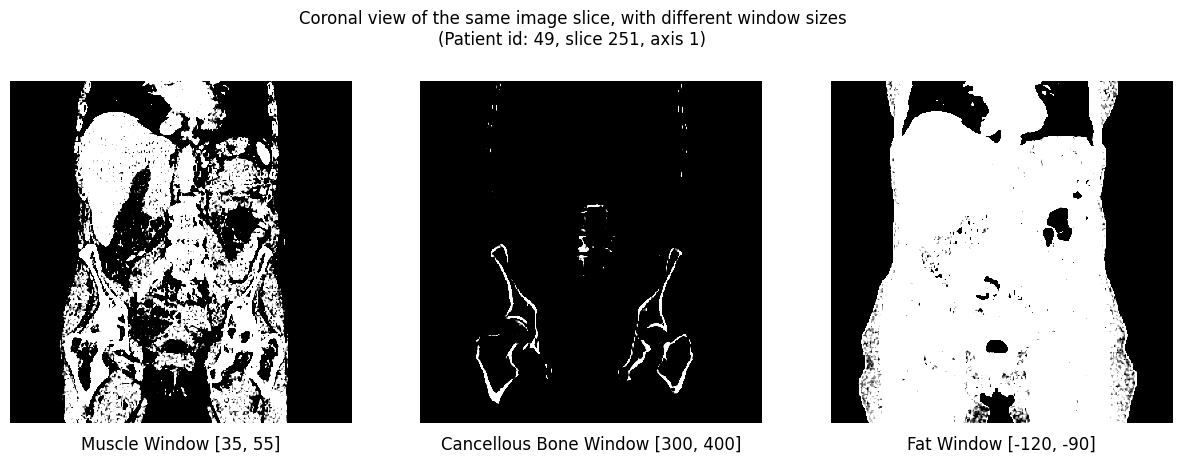
\includegraphics[width=0.3\textwidth, trim=0.2cm 1cm 21cm 2cm, clip]{../figures/HU-window.png}}}
    \subfigure[Cancellous Bone Window  $(300,400)$~\cite{cancellous-bone}]{{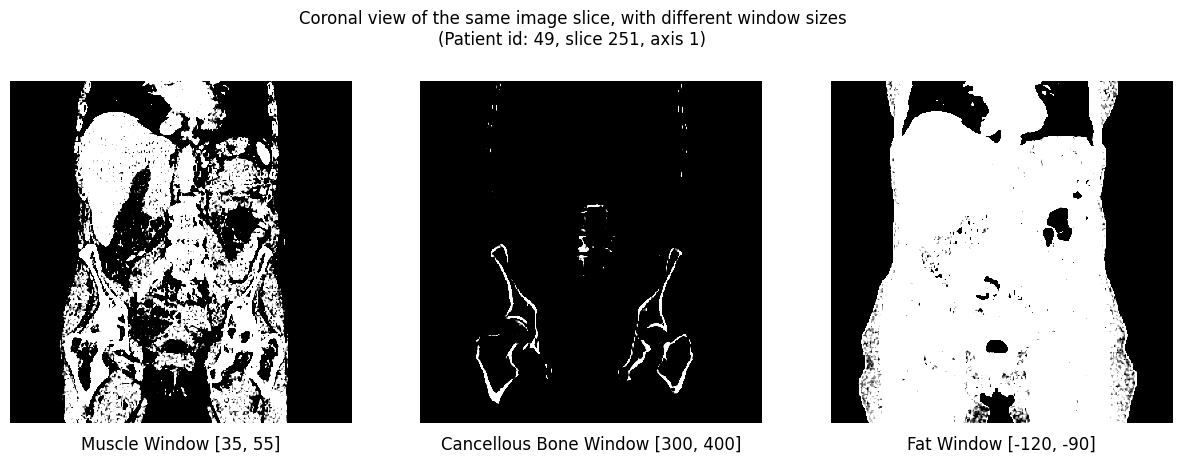
\includegraphics[width=0.3\textwidth, trim=10.6cm 1cm 10.6cm 2cm, clip]{../figures/HU-window.png}}}
    \subfigure[Fat Window $(-120, -90)$~\cite{other-HD-units}]{{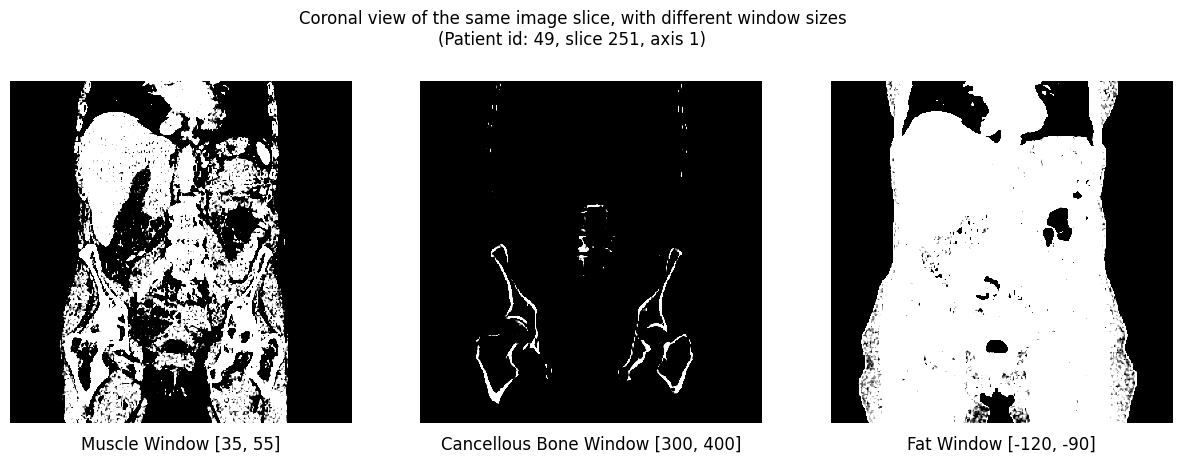
\includegraphics[width=0.3\textwidth, trim=21cm 1cm 0.2cm 2cm, clip]{../figures/HU-window.png}}}
    \caption{Coronal view the same image slice of a CT image, with different window cropping (Patient id: 49, slice 251, axis 1)}
    \label{fig:ct-windows}
\end{figure}

The granularity or image slice thickness is decided by the operator or physician and ranges from 1mm to 10mm. Therefore, the precision along each axis creates a cube, or voxel which represents the value on a grid in three-dimensional space. The voxel values are measured in Hounsfield Units (HU)~\cite{diagnostic-radiology-physics}. 

Contrary to natural images, where pixel values vary from 0 to 255 in 3 channels representing Red, Blue and Green, the Hounsfield scale is a quantitative scale for describing radiodensity where the image intensity reflects tissue type; each voxel intensity refers to specific tissue composition. The positive values are a consequence of more dense tissue with greater X-ray beam absorption, and negative values are less dense tissue with less X-ray beam absorption~\cite{Statpearls}.  

Therefore, becuase the HU scale is relative, different windows may be taken of a CT scan to highlight different tissues. Those voxels that lie within the window, are likely to be tissues of a specific classification. For example, disaplyed in Figure~\ref{fig:ct-windows} we display 3 such windows, muscle, cancellous bone and fat.

\subsection{Data Aquisition}

\subsubsection{Format}

The data acquired through The Royal Marsden Hospital is presented as a set of `Neuroimaging Informatics Technology Initiative' files (NIfTI)~\cite{file-formats}. It serves as a lightweight alternative to other formats such as DICOM and eliminates ambiguity from spatial orientation information~\cite{dicom-to-nifti-conversion}. Libraries exist for handling these files, such as SimpleITK~\cite{SimpleITK-paper} which we use to read and manipulate the data in this project. The library reads, manipulates, and handles the image as a set of points in a grid occupying a physical region in space as defined by the metadata to remove ambiguity from the origin, size, spacing and so on that might vary between patient scans.

\subsubsection{Training Data}

Data was sampled for 100 varying female patients with similar types of cancer. With this data, come 7 relevant segmentation classes which contribute to radiotherapy planning. For the purpose of reproducibility, all delinated lablled data was lablled consistently by the Oncologists to improve chances that an AI model can learn cervical cancer patterns~\cite{AMLART-data}. 

Finally, 10 hold-out data items were provided, which are patients with only the raw CT scan information with no labels.

\subsubsection{Notes}

Some notes contain clinical observations about each of the 100 labelled data pairs~\cite{AMLART-data}. This small sample size of patients is also a good representation of the variability of data in the population. Because of the relatively small sample size, its important to be more acutely aware of the variability in the data. In particular, some observations are summarized.

A common observation is that scans contain poor contrast. For patient 13, the note reads ``no contrast - hard to see LNs'' which is information crutial to determine for segmenting the Clinical Target Volume for Lymph Nodes (CTVn). Additionally, patients 9, 60, and 62 are examples that have ``very large tumors'', sometimes, these even shift into uncommon areas, with ``sigmoid hanging into parametrium''. % GTV not visible?

The notes are helpful to identify and diagnose some reasons for poor performance of the model which is characteristic of the high variability between patients.

\subsection{Delineation classes}

The clinicians at the Royal Marsden Hospital have provided segmentation labels for 5 high-priority classes of interest. These are the Bladder, Anorectum, CTVn, CTVp, and Parametrium.

\subsection{Organs At Risk}\label{sec:data-organs-at-risk}

\begin{figure}[H]
  \centering
  \subfigure[Axial]{
    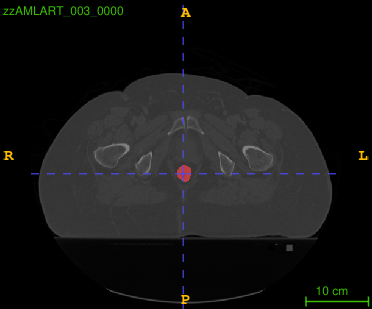
\includegraphics[width=0.3\textwidth]{../figures/PatientStructureExamples/Anorectum_003/Axial.png}
   \label{fig:example-anorectum-axial}
  }
  \subfigure[Coronal]{
    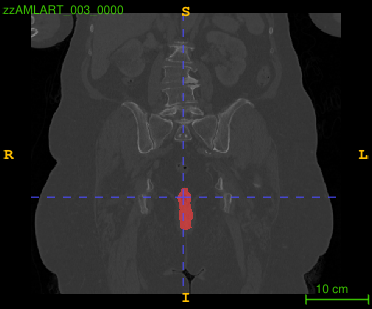
\includegraphics[width=0.3\textwidth]{../figures/PatientStructureExamples/Anorectum_003/Coronal.png}
   \label{fig:example-anorectum-coronal}
  }
  \subfigure[Sagittal]{
    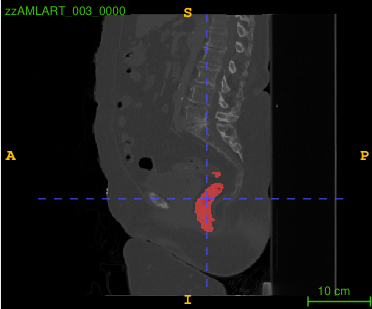
\includegraphics[width=0.3\textwidth]{../figures/PatientStructureExamples/Anorectum_003/Sagittal.png}
   \label{fig:example-anorectum-sagittal}
  }
  \vspace{1em}
  \subfigure[Axial]{
    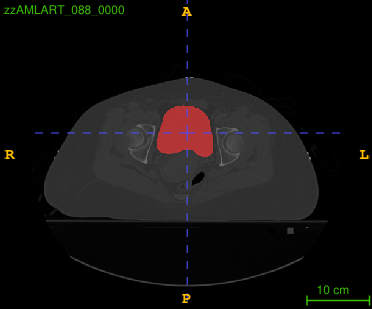
\includegraphics[width=0.3\textwidth]{../figures/PatientStructureExamples/Bladder_088/Axial.png}
   \label{fig:example-bladder-axial}
  }
  \subfigure[Coronal]{
    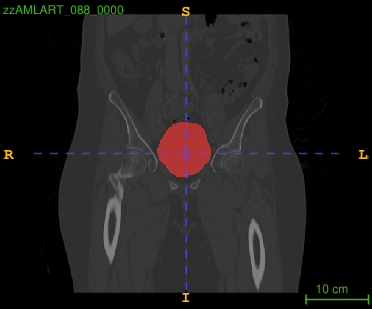
\includegraphics[width=0.3\textwidth]{../figures/PatientStructureExamples/Bladder_088/Coronal.png}
   \label{fig:example-bladder-coronal}
  }
  \subfigure[Sagittal]{
    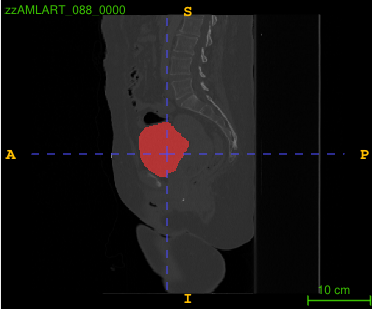
\includegraphics[width=0.3\textwidth]{../figures/PatientStructureExamples/Bladder_088/Sagittal.png}
   \label{fig:example-bladder-sagittal}
  }
  \caption{Views of a segmented (in red) Anorectum (\ref{fig:example-anorectum-axial}-\ref{fig:example-anorectum-sagittal}) and Bladder (\ref{fig:example-bladder-axial}-\ref{fig:example-bladder-sagittal}) of an arbitrary patient}
\end{figure}

An organ at risk is an organ which has a substantial probability of being within the PTV despite being healthy. Any areas that are created around the area should actively avoid these organs because by overlapping with them we risk complicating the treatment and compromising the health of functioning organs.

Many anatomies have been provided in the risk categories, however, in particular we have been supplied with contours for the Bladder (Figure~\ref{fig:example-bladder-axial}-\ref{fig:example-bladder-sagittal}) and the Anorectum (Figure~\ref{fig:example-anorectum-axial}-\ref{fig:example-anorectum-sagittal}). In particular, clinicians have identified that the Bladder may overlap with the CTVn (Section~\ref{sec:data-CTVn}) and the Parametrium (Section~\ref{sec:data-Parametrium}).

\subsection{CTVp}\label{sec:data-CTVp}

\begin{figure}[H]
  \centering
  \subfigure[Axial]{
    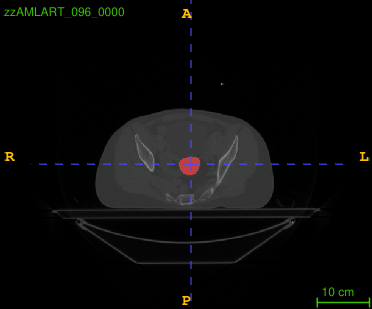
\includegraphics[width=0.3\textwidth]{../figures/PatientStructureExamples/CTVp_096/Axial.png}
   \label{fig:example-CTVp-axial}
  }
  \subfigure[Coronal]{
    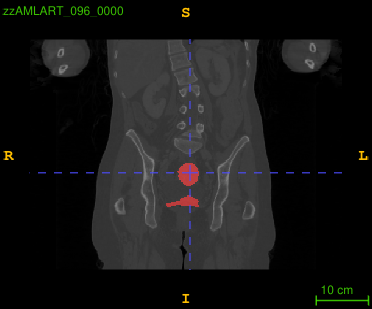
\includegraphics[width=0.3\textwidth]{../figures/PatientStructureExamples/CTVp_096/Coronal.png}
   \label{fig:example-CTVp-coronal}
  }
  \subfigure[Sagittal]{
    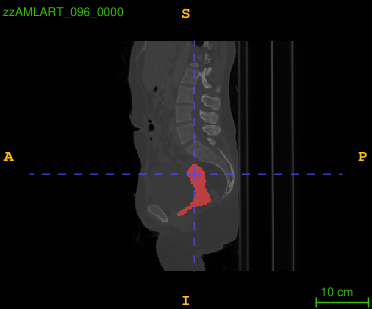
\includegraphics[width=0.3\textwidth]{../figures/PatientStructureExamples/CTVp_096/Sagittal.png}
   \label{fig:example-CTVp-sagittal}
  }
  \caption{Views of a segmented (in red) CTVp of an arbitrary patient}
 \label{fig:example-CTVp}
\end{figure}

The CTVp stands for the Primary Clinical Target Volume, see the example at Figure~\ref{fig:example-CTVp}. This is the CTV where there may be local microscopic spread (uterus, cervix, upper vagina, primary tumour)~\cite{AMLART-data}. This is the area that contains the tumour.

This isn't by any means an organ in a body, but rather an area comprised of other components formed by joining other structures together. The CTVp is an area defined in Equation~\ref{eq:ctvp}.

\subsection{CTVn}\label{sec:data-CTVn}

\begin{figure}[H]
  \centering
  \subfigure[Axial]{
    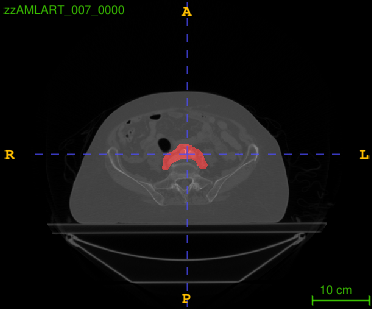
\includegraphics[width=0.3\textwidth]{../figures/PatientStructureExamples/CTVn_007/Axial.png}
   \label{fig:example-CTVn-axial}
  }
  \subfigure[Coronal]{
    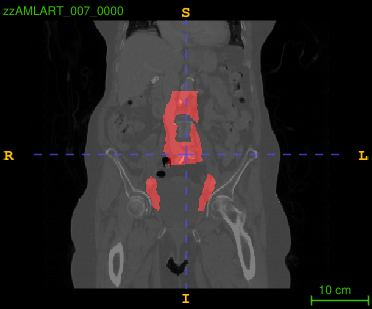
\includegraphics[width=0.3\textwidth]{../figures/PatientStructureExamples/CTVn_007/Coronal.png}
   \label{fig:example-CTVn-coronal}
  }
  \subfigure[Sagittal]{
    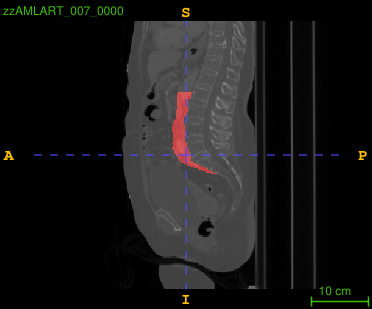
\includegraphics[width=0.3\textwidth]{../figures/PatientStructureExamples/CTVn_007/Sagittal.png}
   \label{fig:example-CTVn-sagittal}
  }
  \caption{Views of a segmented (in red) CTVn of an arbitrary patient}
 \label{fig:example-CTVn}
\end{figure}

The CTVn stands for Nodal Clinical Target Volume, see the example at Figure~\ref{fig:example-CTVn}. This is the CTV where there may be microscopic spread to lymph nodes. It is drawn based on set margins around pelvic blood vessels and includes pelvic lymph nodes, common iliac lymph nodes and para-aortic lymph nodes~\cite{AMLART-data}.

Similarly to CTVp, this is a compound area with three groups of lymph nodes. In clinical practice, the number of these groups included in the CTV varies in each patient, depending on how advanced the disease is. Pathological lymph nodes (GTVn) are also included. The CTVn is an area defined in Equation~\ref{eq:ctvn}.

\subsection{Parametrium}\label{sec:data-Parametrium}

\begin{figure}[H]
  \subfigure[Axial]{
    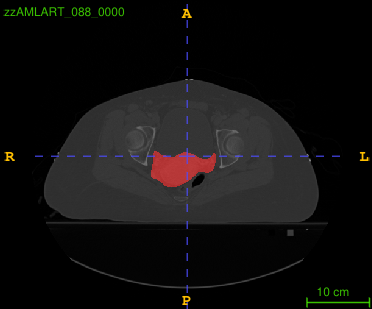
\includegraphics[width=0.3\textwidth]{../figures/PatientStructureExamples/Parametrium_088/Axial.png}
   \label{fig:example-Parametrium-axial}
  }
  \subfigure[Coronal]{
    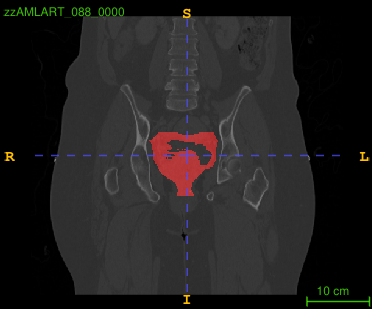
\includegraphics[width=0.3\textwidth]{../figures/PatientStructureExamples/Parametrium_088/Coronal.png}
   \label{fig:example-Parametrium-coronal}
  }
  \subfigure[Sagittal]{
    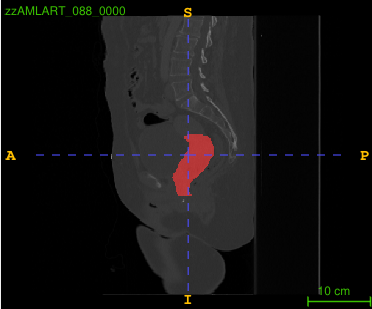
\includegraphics[width=0.3\textwidth]{../figures/PatientStructureExamples/Parametrium_088/Sagittal.png}
   \label{fig:example-Parametrium-saggital}
  }
  \caption{Views of a segmented (in red) Parametrium of an arbitrary patient}
 \label{fig:example-Parametrium}
\end{figure}

The Parametrium (or Paravagina) is the tissue surrounding the cervix/vagina - at risk of local spread, see Figure~\ref{fig:example-Parametrium}. Drawn as a complete structure and editing back to the level of vagina to be included~\cite{AMLART-data}.

\section{Establishing Rules for Structures}\label{sec:data-delineation-rules}

\begin{minipage}{0.5\textwidth}
  \subsubsection{Notation of Structures}
  \begin{enumerate}
    \item Let the Anorectum be denoted as $A$
    \item Let the Bladder be denoted as $B$
    \item Let the Cervix be denoted with $C$
    \item Let the CTVn be denoted with $C_n$
    \item Let the CTVp be denoted with $C_p$
    \item Let the GTVp be denoted with $G_p$
    \item Let the GTVn be denoted with $G_n$
    \item Let the Pelvic Lymph Node be denoted as $L_p$
    \item Let the Common Iliac Lymph Node be denoted as $L_i$
    \item Let the Para-aortic Lymph Node be denoted as $L_{pa}$
  \end{enumerate}
\end{minipage}%
\begin{minipage}{0.5\textwidth}

  \begin{enumerate}
    \setcounter{enumi}{10}
    \item Let the Parametrium be denoted with $P$
    \item Let the Uterus be denoted with $U$
    \item Let the Vagina be denoted with $V$
  \end{enumerate}

  \subsection{Relationship between Structures}

  \begin{enumerate}
    \item Let $O$ denote the set $O = \{B, A, C_n, C_p, P \}$ for a particular patient. If we want to talk about a specific patient, we should use the super-script notation to differentiate patients, e.g., $O^i = \{B^i, A^i, C_n^i, C_p^i, P^i\}$.
    \item Let the overlap of two structures be denoted by the set intersect symbol $\cap$.
    \item Let the joint area of two structures be denoted by the set union symbol $\cup$.
  \end{enumerate}

  % \vspace{4em}

\end{minipage}

\subsection{Rules}

The top 5 priority structures have been selected to identify and plan an area where radiotherapy should be used. With these structures, there are rules that the clinicians have outlined, they are quoted for clarification (these structures only refer to each independent patient):

\begin{enumerate}
  \item There should be no overlap between the CTVn, CTVp or Anorectum.

        \begin{equation}
          \forall{i,j \in \{C_n, C_p, A\}}\text{ with } i \neq j, i \cap j = \emptyset
        \end{equation}

  \item The Parametrium may overlap with all of the other structures.

        \begin{equation}
          \forall i \in S, \quad P \cap S_i \neq \emptyset \quad \text{(Possibly)}
        \end{equation}

  \item The Bladder may overlap with the CTVn.

        \begin{equation}
          B \cap C_n \neq \emptyset \vee B \cap C_n = \emptyset\label{eq:ctvn}
        \end{equation}

  \item The CTVp is defined as a compound structure containing:

        \begin{equation}
          C_p = \overbrace{C \cup G_p}^{\text{High Risk CTV}} \quad \cup \quad U \cup V\label{eq:ctvp}
        \end{equation}

  \item The CTVn is defined as a compound structure containing:

        \begin{equation}
          C_n = G_n \cup L_i \cup L_p + L_{pa}
        \end{equation}

\end{enumerate}

\section{Technical Context}
\subsection{AI in medical imaging}
\subsection{nnUNet}
\subsection{TotalSegmentator}
\subsection{UniverSeg}
\subsection{SAM}

%%%%%%%%%%%%%%%%%%%%%%%%%%%%%%%%%%%%
\chapter{Methodology}

\section{Evaluation Metrics}
\section{Base-line nnUNet...}

%%%%%%%%%%%%%%%%%%%%%%%%%%%%%%%%%%%%
\chapter{Results}

%%%%%%%%%%%%%%%%%%%%%%%%%%%%%%%%%%%%
\chapter{Discussion}

%%%%%%%%%%%%%%%%%%%%%%%%%%%%%%%%%%%%
\chapter{Conclusion}

%%%%%%%%%%%%%%%%%%%%%%%%%%%%%%%%%%%%
\chapter{Ethics}

The lack of effort to protect the identities and confidentiality of patients during research projects may result in ``stigma, embarrassment, and discrimination''~\cite{health-privacy} if the data is misused.
This project involves very intimate and personal information of many female patients whose privacy must be established concretely before research is to take place.%. Researchers may collaborate with third-parties such as Imperial College London by providing anonymized data which may not be reverse engineered back to the patient.

\section{Patient disclosures}

Reserachers may collaborate with third-parties such as Imperial College London by providing anonymized data which may not be reverse engineered back to the patient. The collaborating hospital, The Royal Marsden Hospital, doesn't require ``explicit consent'' for sharing collected clinical data with outside entities as long as the patient is made aware of the ways their ``de-identified/anonymized'' data may be used.~\cite{royal-marsden-privacy-note}. Formalities are also arranged with Imperial Collage's Medical Imaging team such as acting as ``ethical data stewards''~\cite{Larson2020-ib}. Without such disclosure and anonymisation of data, patients may be reluctant to provide candid and complete disclosures of their sensitive information, even to physicians, which may prevent a full diagnosis if their data isn't maintained in an anonymous fashion.

The MIRA team acts as responsible data stewards by storing anonymized data within a folder on the college network. All provided data was anonymized by the Royal Marsden Hospital and sent to team MIRA in the \texttt{NIfTI} file format which discloses no personal identifiable information, as defined by GOV website~\cite{gov-gdpr}. This folder contains security measures which limit the availability of data only to those with specific access rights. Furthermore, operating on the preamble of de-identified data further reduces individual patient risk in the event that data is ever brought outside the confines of this folder.

\section{Using the tool}\label{sect:using-the-tool}

The applications of this tool bode well in the healthcare ecosystem as the community slowly accepts the involvement of AI-powered medical tools. Radiology has been one application that has been most welcoming of the new advances in technology as there is potential for substantial aid by reducing manual labor, increasing precision and freeing up the primary care physician's time~\cite{Amisha2019-ki}.

Yet, it is too early to take result the medical tool as gospel. For current cervical radiotherapy delineation tools, only 90\% of the output is considered as acceptable for clinical use~\cite{LIU2020172}. The remainder therefore has the potential to cause more harm than good if not checked properly. For example, overlap of a PTV onto an organ-at-risk may invoke a cascade of negative effects for the patient. A physician may base their final judgement subject to a multivariate analysis, which is contrary to the single image modality that this tool is based on. Therefore, the tool should be used as a second opinion rather than a primary source of information.

Clinicians can fall into the trap of automation-bias as AI becomes more common place in clinical environments~\cite{STRAW2020101965}. However, many models of this age codify the existing bias in common cases, which often will fail those patients who do not fit the expectations of the majority. Therefore, a degree of supervision required from physicians has to be established if this tool is to be used in practice. Oncologists will be required to reverse-engineer results of the `black-box' to verify why a decision has been made. Secondly, the responsible party for incorrect decisions made by DL tools should also be determined~\cite{Chen2021-dg}.

%%%%%%%%%%%%%%%%%%%%%%%%%%%%%%%%%%%%

%% bibliography
\bibliography{../.latex-templates/references}

\end{document}